\documentclass[aps,prb,superscriptaddress,nofootinbib]{revtex4}
\usepackage{amsfonts}
\usepackage{amsmath}
\usepackage{amssymb}
\usepackage{graphicx}
\usepackage{graphbox}
\usepackage{caption}
\usepackage{bm}
\usepackage{bbm}
\usepackage{cancel}
\usepackage{color}
\usepackage{mathrsfs}
\usepackage[colorlinks,bookmarks=true,citecolor=blue,linkcolor=red,urlcolor=blue]{hyperref}
\usepackage{simpler-wick}
\usepackage{appendix}
\usepackage{float}
\usepackage{sleek-listings}
\usepackage{array}
\usepackage{booktabs}
\setlength{\parindent}{10 pt}
\setlength{\parskip}{2 pt}
\setcounter{MaxMatrixCols}{30}
\bibliographystyle{apsrev}

\newcommand{\normord}[1]{{:\mathrel{#1}:}}
\def\tbs{\textbackslash}
\def \tr{\operatorname{tr}}
\def \Tr{\operatorname{Tr}}


\begin{document}
\title{Phi-4 Theory}
\author{Jie Ren}

\FrameTBStyle{mathematica}

\maketitle



In this chapter, we study the interacting scalar field theory $\mathcal L = \mathcal L_0 + \mathcal L_{\mathrm{int}}$.
The free field part is assumed to be Klein-Gordon field 
\begin{equation}
	\mathcal L_0 =\frac{1}{2}\partial^\mu \phi \partial_\mu \phi -\frac{m^2}{2}\phi^2.
\end{equation}
Assuming the theory has the reflection symmetry: $\phi \rightarrow -\phi$, the simplest form of interaction is the quartic term $\mathcal L_{\mathrm{int}} = -\frac{g}{4!}\phi^4$.
Such theory is called the $\phi^4$ theory.
In this note, we discuss two renormalization scheme for the $\phi^4$ theory, and discuss the spontaneous symmetry breaking.


\tableofcontents



\section{Perturbative Renormalization}

As the result of the interaction, the field and coefficients will be renormalized:
\begin{equation}
	\phi = \sqrt{Z_\phi} \phi_R, \quad
	m = \sqrt{Z_m} m_R, \quad
	g = Z_g g_R.
\end{equation}
The renormalized Lagrangian can be formally divided into three parts: 
\begin{equation}
\begin{aligned}
	\mathcal{L} &= Z_\phi \frac{1}{2} (\partial_\mu\phi_R)^2 - Z_m Z_\phi \frac{m_R^2}{2} \phi_R^2 - Z_g Z_\phi^2 \frac{g_R}{4!}\phi_R^4 \\
	&= \mathcal L_0 + \mathcal L_{\mathrm{int}} + \mathcal L_{\mathrm{ct}}.
\end{aligned}
\end{equation}
The free and interaction part is chosen to be the same as the original theory, while we have introduced additional counter term:
\begin{equation}
	\mathcal L_{\mathrm{ct}} = A \frac{1}{2} (\partial_\mu\phi_R)^2 - B\frac{ m_R^2}{2} \phi_R^2 - C \frac{g_R}{4!} \phi_R^4
\end{equation}
with coefficients (formally infinite which is used to cancel the divergence from the loop corrections):
\begin{equation}
	A = Z_\phi-1, \quad 
	B = Z_m Z_\phi - 1, \quad 
	C = Z_g Z_\phi^2 - 1.
\end{equation}
The counter terms will be treated as additional perturbations.


\subsection{First-order Correction to the Propagator}
Consider the first order perturbation to the propagator:
\begin{equation}
\begin{aligned}
	i \Delta^{(1)}(k)
	&= 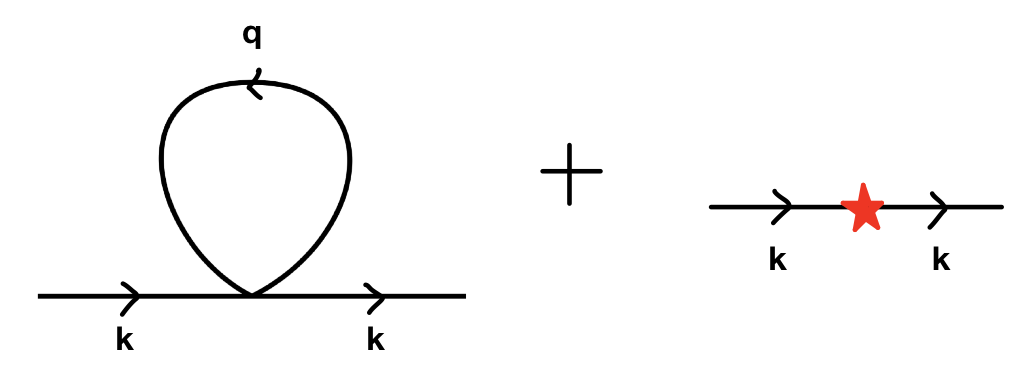
\includegraphics[align=c, width=0.35\linewidth]{pics/KG-3.png} \\
	&= i\Delta_0(k) \left[-\frac{g}{2}\int \frac{d^4 q}{(2\pi)^4} \frac{1}{q^2-m_R^2} + i(Ak^2-Bm_R^2) \right] i\Delta_0(k).
\end{aligned}
\end{equation}
Note that in the loop diagram, there is in total ($4 \times 3 = 12$) identical diagrams, and so gives the coefficients.
A simpler counter rule is that if the diagram has no symmetry, there is in total $4!$ identical diagrams and the denominator cancels out exactly, while for any remaining symmetries, the symmetry factor will remain in the denominator.
For the loop diagram we considered here, the symmetry factor is $2$.

Note that the second order correction to the Green's function has one ``ingoing'' leg and one ``outgoing'' leg, the core (or the amputated Green's function) in this case is called the \textit{self-energy} $i\Sigma(k^2)$:
\begin{equation}
	i\Sigma(k^2) = -\frac{g}{2}\int \frac{d^4 q}{(2\pi)^4} \frac{1}{q^4-m_R^2} + i(Ak^2-Bm_R^2).
\end{equation}
The integral is divergent, that when the counter terms come to rescue.
The divergent part of the integral can be absorbed into the coefficients, or be canceled by the counter terms.
In the following, we will see that the divergent integral
\begin{equation}
	I \equiv -\frac{g}{2} \int \frac{d^4 q}{(2\pi)^4} \frac{1}{q^4-m_R^2}
\end{equation}
can be regularized.
The regularization is typically controlled by a parameter which will recover the infinity when taking a specific limit.
The physical observable shall not depend explicitly on the regularization parameter, so the final result is free from divergent even if we take the limit.


\subsubsection{Regularization of the Divergent Integral}
Consider the integral
\begin{equation}
	I = -\frac{g}{2} \int\frac{d \omega}{2\pi} \int\frac{d^3 q}{(2\pi)^3} \frac{1}{\omega^2 - \bm q^2-m_R^2 -i\varepsilon}.
\end{equation}
Since the singularity locates at $\pm(\sqrt{\bm q^2+m_R^2}-i\varepsilon)$, we can analytically change the integral of $\omega$ from real axis to the imaginary axis anti-clock-wisely, the result is equivalent to the substitution $\omega \rightarrow i\omega$.
The new integral is defined on the 4D Euclidean space:
\begin{equation}
	I = i \frac{g}{2} \int \frac{d^4 q}{(2\pi)^4} \frac{1}{q^2 + m_R^2}
	= i\frac{g}{2} \frac{\Omega_4}{(2\pi)^4} \int_0^\infty dq \ \frac{q^3}{q^2 + m^2_R},
\end{equation}
where $\Omega_d = 2 \pi^{d/2}/\Gamma\left(d/2\right)$ is the $d$-dimensional spherical area.

Till now the integral is essentially the same and thus still divergent.
Now we are going to regularize the expression.
One most frequently used regularization scheme is the \textit{dimensional regularization}.
It take note of the fact that the divergence of the integral only happens at integer dimension.
When we put the field theory to ($d=4-\varepsilon$)-dimensional space, the integral becomes:
\begin{equation}
	I_\varepsilon = i\frac{g\tilde{\mu}^\varepsilon}{2}\frac{\Omega_{4-\varepsilon}}{(2\pi)^{4-\varepsilon}} \int_0^\infty dq\ \frac{q^{3-\varepsilon}}{q^2+m_R^2}.
\end{equation}
Note that we have introduced a mass scale $\tilde\mu$ to get the correct dimensionality.
The integral is now convergent.
The specific form the the integral is not important, but we are concerned about the expansion near $\varepsilon = 0$. 
All the computation here can be done automatically (in \texttt{Mathematica}), and the result is
\begin{equation}
\begin{aligned}
	I_\varepsilon &= i\frac{g m_R^2}{32\pi^2} \left[\frac{2}{\varepsilon}+1+\log \left(\frac{4 \pi \tilde{\mu}^2 e^{-\gamma_E}}{m_R^2}\right)\right] + O(\varepsilon) \\
	&\equiv i\frac{g m_R^2}{32\pi^2} \left[\frac{2}{\varepsilon}+1+\log \left(\frac{\mu^2}{m_R^2}\right)\right] + O(\varepsilon),
\end{aligned}
\end{equation}
where $\gamma_E$ is the Euler constant. 
We have seen that the integral is controlled by the parameter $\varepsilon$.
In the $\varepsilon \rightarrow 0$ limit, the integral is divergent.


\subsubsection{Renormalization Using the Counter Terms}
We are now going to renormalize the theory.
Note that in the self-energy definition
\begin{equation}
	\Sigma(k^2) = \frac{1}{i} I + A k^2-B^2 m_R^2,
\end{equation}
we have the freedom to choose the counter terms that cancel the infinity.
To the first order, the coefficients can be
\begin{equation}
	A = O(g^2), \quad
	B = \frac{g}{16\pi^2 \varepsilon} + O(g^2).
\end{equation}
The result is
\begin{equation}
	\Sigma(k^2) = \frac{g m_R^2}{16\pi^2} \log \left(\frac{\mu}{m_R}\right)
	+\frac{g m_R^2}{32\pi^2}+O(\varepsilon).
\end{equation}
The one-loop correction also leads to a infinite \textit{Dyson series}:
\begin{equation}
\begin{aligned}
	i\Delta(k) &= i\Delta_0(k) + i\Delta_0(k)\sum_{n=1}^\infty \left[i\Sigma(k^2)i\Delta_0(k)\right] \\
	&= \frac{i}{k^2 -m_R^2 + \Sigma(k^2)}.
\end{aligned}
\end{equation}



\subsubsection{Physical Observables}
The physical observable here is the rest mass $m_0$, which is experimentally measurable.
It equals to the pole of the propagator, i.e.,
\begin{equation}
	m_R^2 - \Sigma(m_0^2) = m_0^2.
\end{equation}
Depending on the mass scale $\mu$ we choose, the renormalized mass $m_R$ may or may not equal to the rest mass.
Specifically, we can choose mass scale so that $m_R = m_0$, that is
\begin{equation}
	\Sigma(m_0^2) = 0 \quad \Longrightarrow \quad
	\mu = e^{-\frac{1}{2}} m_0.
\end{equation}
To the first order, the self-energy has no momentum dependence, so there is no physical prediction.




\subsection{Second-order Correction to the Vertex}

Now consider the second order correction to the vertex function, which is the connected, amputated 4-point Green's function.
The perturbation correspond to 3 different Feynman diagrams together with a vertex counter term.
The explicit form is: 
\begin{equation}
\begin{aligned}
	i\Gamma_4(k_1,k_2,k_3,k_4) 
	&= 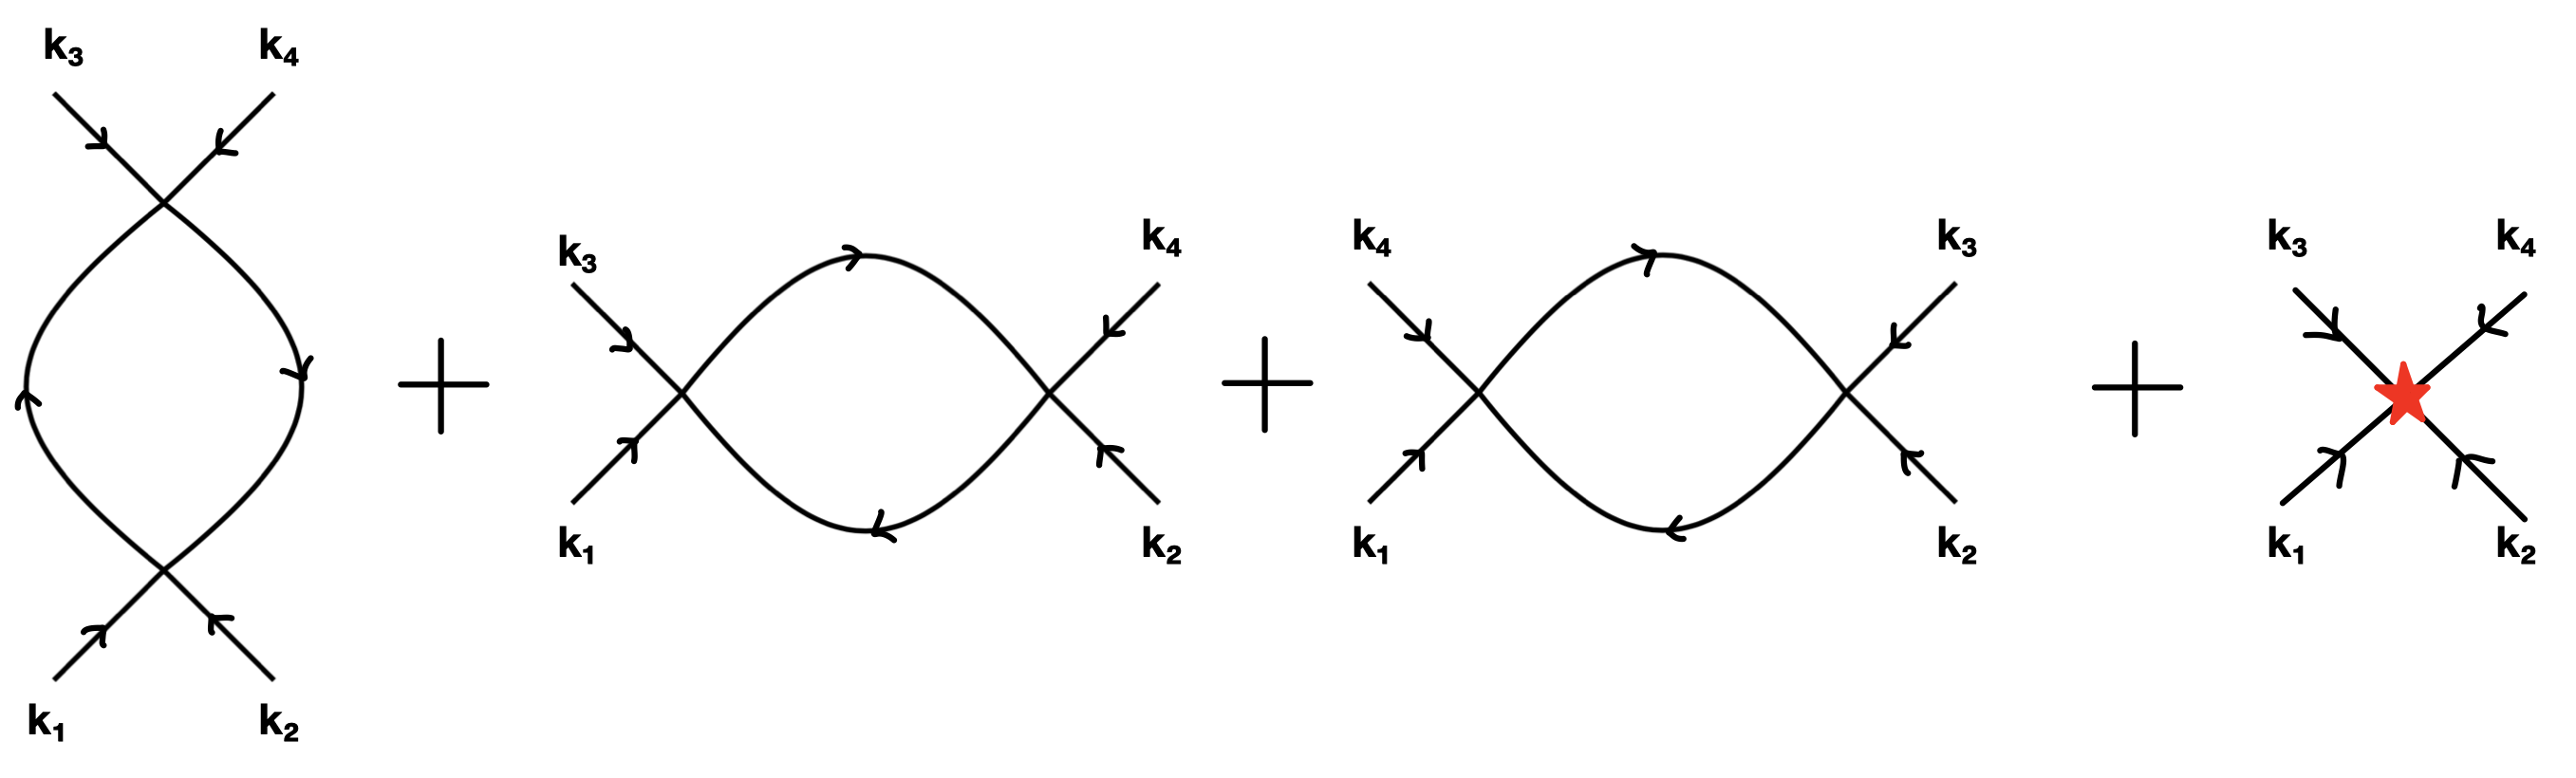
\includegraphics[align=c, width=0.6\linewidth]{pics/KG-4.png}\\
	&= \frac{g_R^2}{2} \left[iF(s)+iF(t)+iF(u)\right] -iCg_R,
\end{aligned}
\end{equation}
where we have introduced three momentum parameters $s$, $t$, and $u$: 
\begin{equation}
	s = (k_1+k_2)^2,\quad
	t = (k_1+k_3)^2,\quad
	u = (k_1+k_4)^2.
\end{equation}
The loop integrals for three channels are the same, denoted by
\begin{equation}
	iF(k^2) = \int \frac{d^4 q}{(2\pi)^4} \Delta_0(q) \Delta_0(q+k).
\end{equation}
The integral is again divergent.



\subsubsection{Regularization}
The denominator in the integral
\begin{equation}
	iF(k^2) = \int \frac{d^4 q}{(2\pi)^4} \frac{i}{q^2-m_R^2} \frac{i}{(q+k)^2-m_R^2}
\end{equation}
involves multiplication of two polynomial.
The expression can be simplified by the \textit{Feynman parametrization}, which is essentially the identity:
\begin{equation}
	\frac{1}{A_{1} \ldots A_{n}}=\int d F_{n}\left(x_{1} A_{1}+\ldots+x_{n} A_{n}\right)^{-n},
\end{equation}
where the integration measure over the Feynman parameters $x_{i}$ is
\begin{equation}
	\int d F_{n}=(n-1) ! \int_{0}^{1} d x_{1} \ldots d x_{n} \delta\left(x_{1}+\ldots+x_{n}-1\right).
\end{equation}
This measure is normalized so that $\int d F_{n} =1$. 
The simplest case is
\begin{equation}
	\frac{1}{A B}=\int_{0}^{1} \frac{dx}{[A+(B-A) x]^{2}}
	=\int_{0}^{1} \frac{\delta(x+y-1)}{[x A+y B]^{2}} dx dy.
\end{equation}
Other useful identities are
\begin{equation}
\begin{aligned}
	\frac{1}{A B^{n}} &=\int_{0}^{1} dxdy\frac{\delta(x+y-1)n y^{n-1}}{[x A+y B]^{n+1}} , \\
	\frac{1}{A B C} &=\int_{0}^{1} dxdydz \frac{2\delta(x+y+z-1)}{[x A+y B+z C]^{3}} .
\end{aligned}
\end{equation}

Using the Feynman parameters, the integral is
\begin{equation}
	iF(k^2) = \frac{i\Omega_4}{(2\pi)^4} \int_0^1 dx \int dq\ \frac{q^{3}}{\left[q^2+m_R^2+x(1-x)k^2\right]^2}.
\end{equation}
Using the dimensional regularization, the integral is
\begin{equation}
	iF_\varepsilon(k^2) = \frac{i\tilde{\mu}^{\varepsilon}\Omega_{4-\varepsilon}}{(2\pi)^{4-\varepsilon}} \int_0^1 dx \int dq\ \frac{q^{3-\varepsilon}}{\left[q^2+m_R^2+x(1-x)k^2\right]^2}.
\end{equation}
Then we carry out the calculation, the result is:
\begin{equation}
\begin{aligned}
	F_\varepsilon(s) &= \frac{1}{8\pi^2\varepsilon} + \frac{1}{16\pi^2}\int_0^1 dx \ln \left(\frac{4\pi \tilde{\mu}^2 e^{-\gamma_E}}{D_{s,x}}\right) \\
	&= \frac{1}{8\pi^2\varepsilon} +\frac{1}{8\pi^2}\ln \left(\frac{\mu}{m_R}\right) - \frac{1}{16\pi^2}\int_0^1 dx \ln\left(\frac{D_{s,x}}{m_R^2}\right),
\end{aligned}
\end{equation}
where we have denote
\begin{equation}
	D_{k^2,x} \equiv m_R^2+x(1-x)k^2.
\end{equation}
Now sum up the contribution from all channel, the result looks like:
\begin{equation}
	\Gamma^{(2)}_4 = \frac{3 g_R^2}{16\pi^2}\left[\frac{1}{\varepsilon} + \ln\left(\frac{\mu}{m_R}\right)\right] - \frac{g_R^2}{32\pi^2}\int_0^1 dx \ln\left(\frac{D_{s,x}D_{t,x}D_{u,x}}{m_R^6}\right)- C g_R.
\end{equation}


\subsubsection{Renormalization and Physical Observables}

To absorb the divergence, we can choose the counter term coefficient as
\begin{equation}
	C = \frac{3g_R}{16\pi^2}.
\end{equation}
So, to the second order, the vertex function is:
\begin{equation}
	\Gamma_4(k_1,k_2,k_3,k_4) = -g_R + \frac{g_R^2}{32\pi^2}\int_0^1 dx \ln\left(\frac{\mu^6}{D_{s,x}D_{t,x}D_{u,x}}\right).
\end{equation}
The vertex function is directly related to the physical observables.
It can be measured in the scattering experiment or just just by the repulsive force it generated.
We can choose the scale $\mu_0$ so that
\begin{equation}
	\Gamma(m_R,m_R,m_R,m_R) = -g_R.
\end{equation}
Then the corrected vertex function gives the physical predictions, for example on the scattering amplitude for different $k_i$'s.

\subsection{Renormalization Group}
Now consider the RG equation for the one-loop correction. 
The bare parameters are:
\begin{equation}
	g_0 = Z_g g\tilde{\mu}^{\varepsilon},\ 
	m_0 = Z_m^{1/2} m,
\end{equation}
The RG conditions are:
\begin{eqnarray}
	\frac{d g_0}{d\ln \mu}
	&=& \left(\frac{3}{16\pi^2 \varepsilon} + \frac{1}{g}\right)\frac{dg}{d\ln \mu} + \varepsilon = 0, \\
	\frac{d m_0}{d\ln \mu}
	&=& \frac{1}{32\pi^2 \varepsilon}\frac{dg}{d\ln \mu} + \frac{1}{m}\frac{dm}{d \ln \mu} = 0.
\end{eqnarray}
Consider the series expansion of beta function:
\begin{equation}
	\beta(g) = \frac{dg}{d\ln \mu} = \beta_1 g + \beta_2 g^2 +O(g^3).
\end{equation}
The beta function is
\begin{equation}
	\beta(g) = -\varepsilon g + \frac{3g^2}{16\pi^2} + O(g^3).
\end{equation}
The anomalous dimension of mass is
\begin{equation}
	\gamma_m = \frac{1}{m}\frac{dm}{d \ln \mu} = \frac{g}{32\pi^2}+O(g^2).
\end{equation}
One noticeable fact is that when we make the analytic continuation to $\varepsilon>0$, the betta function predict a nontrivial fixed point at
\begin{equation}
	g^*_{\mathrm{WF}} = \frac{16\pi^2 \varepsilon}{3}.
\end{equation}
This fixed point is called the \textit{Wilson-Fisher fixed point}, and is related to the ferromagnetic-paramagnetic transition.



\section{Wilsonian Renormalization Group}

In this section, we consider another regulation scheme from Wilson's perspective.
We introduce a UV cutoff for the theory, and the action for $\phi^4$ theory is
\begin{equation}
	S[\phi] = \int_{|k|<\Lambda} \frac{d^d k}{(2\pi)^d}\left[\frac{1}{2} \left(k^2-r(\Lambda)\right)\phi^2 - \frac{1}{4!}g(\Lambda)\phi^4\right].
\end{equation}
We choose to fix the coefficient of the kinetic term.
The mass and coupling constant is dependent of the energy scale $\Lambda$.
The course graining makes $k \rightarrow s k$.
In the momentum domain, we split the field into slow and fast parts $\phi = \phi_{s} + \phi_{f}$, integrate the fast momentum part $\Lambda/s<|k|<\Lambda$, rescale the field strength, and obtain new effective theory.




\subsection{Integral over Energy Shell}

We first consider the one-loop correction:\footnote{In this section, the field theory is defined on the Euclidean space.}
\begin{equation}
	e^{-S'[\phi_{\mathrm{s}}]} = \int D[\phi_{\mathrm{f}}] e^{-S[\phi_{\mathrm{s}}+\phi_{\mathrm{f}}]}.
\end{equation} 
The action can be decomposed into the fast field part, slow field past, and the interacting part:
\begin{equation}
	S[\phi_{\mathrm{s}}+\phi_{\mathrm{f}}] = S[\phi_{\mathrm{s}}] + S[\phi_{\mathrm{f}}] + S[\phi_{\mathrm{s}}, \phi_{\mathrm{f}}].
\end{equation}
In the $\phi^4$ case, the only relevant part of the action is
\begin{equation}
	S[\phi_{\mathrm{s}},\phi_{\mathrm{f}}] = \frac{g}{4} \int d^d x\ \phi_{\mathrm{s}}^2 \phi_{\mathrm{f}}^2 + \cdots
\end{equation}
The effective action for the slow field can be obtained by integrate out the fast field.
To the second order,
\begin{equation}
\begin{aligned}
	\exp\left(-S'[\phi_{\mathrm{s}}]\right) 
	&= e^{-S[\phi_{\mathrm{s}}]} \left[1-\langle S[\phi_{\mathrm{s}},\phi_{\mathrm{f}}]\rangle_f + \frac{1}{2} \langle S[\phi_{\mathrm{s}},\phi_{\mathrm{f}}]\rangle^2+O(g^3) \right]\\
	&= \exp\left[-S[\phi_{\mathrm{s}}]-\langle S[\phi_{\mathrm{s}},\phi_{\mathrm{f}}]\rangle_f + \frac{1}{2}\langle S[\phi_{\mathrm{s}},\phi_{\mathrm{f}}]^2\rangle^c_f +O(g^3)\right].
\end{aligned}
\end{equation}
This produce a new action with different coefficients, and possibly new terms.
In the renormalization group sense, we only need to keep track of the coefficients of the relevant terms.\footnote{Although the irrelevant terms vanishes during the RG flow, they may contributes back to the relevant terms and thus influence the RG flow. However, this process is captured by higher order perturbation theory. So in practice, we just ignore all the diagram producing irrelevant terms.}
After proper renormalization, the coupling constant can alter in the coarse-graining process.


\subsection{RG-Flow of Phi-4 Theory}

The first order perturbation contribute to the mass term:
\begin{equation}
\begin{aligned}
	\left\langle S\left[\phi_{\mathrm{s}}, \phi_{\mathrm{f}}\right]\right\rangle_{\mathrm{f}}
	= 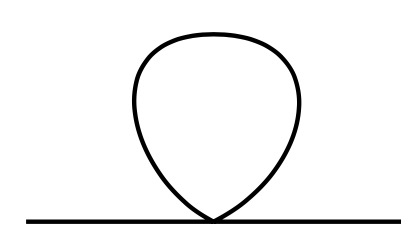
\includegraphics[align=c,width=0.1\linewidth]{pics/RG-1.jpg} 
	=\frac{g}{4} \int_{d\Lambda} \frac{d^d q}{(2 \pi)^d} \frac{1}{r+q^{2}} \int_{|k|<\Lambda/s} \frac{d^d k}{(2 \pi)^{d}} \phi_{\mathrm{s}}(k) \phi_{\mathrm{s}}(-k).
\end{aligned}
\end{equation}
We are interested in the RG-flow in the vicinity of the critical point. 
So we can calculate the coefficient perturbatively for $r$:
\begin{equation}
	\int_{d\Lambda} \frac{d^d q}{(2 \pi)^d} \frac{1}{r+q^{2}}
	= \int_{d\Lambda}\frac{d^d q}{(2 \pi)^d} \left(\frac{1}{q^2} - \frac{r}{q^4}\right)
	= \Omega_d \left[\frac{1-s^{2-d}}{d-2} - \frac{r\left(1-s^{4-d}\right)}{d-4}\right],
\end{equation} 
where $\Omega_{d}=\left(2 \pi^{d / 2} / \Gamma(d / 2)\right) /(2 \pi)^{d} $ denotes the volume of the $d$-dimensional unit sphere.
Note that we used $\Lambda$ as the unit, since it is the only natural scale of the theory.
After the energy-shell integral, we should also renormalize the theory.
To restore the energy shell back to $1$, we change the variable as $k'=sk$, which left an additional $s^{-d-2}$ factor in the kinetic term.
Therefore we renormalize the field as $\phi \rightarrow s^{d/2+1}\phi$.
Take all things into account, and set the infinitesimal variable as $s=e^{dl}$, we get the RG flow of $r$ as
\begin{equation}
\begin{aligned}
	dr &\rightarrow s^2\left[r+\frac{g \Omega_{d}}{2(d-2)}\left(1-s^{2-d}\right)-\frac{r g \Omega_{d}}{2(d-4)}\left(1-s^{4-d}\right)\right]-r \\
	&\simeq (1+2dl) \left[r+ \frac{1}{2} g \Omega_{d} dl - \frac{1}{2} r g \Omega_{d} dl \right]-r \\
	&\simeq \left(2r+ \frac{1}{2}g\Omega_d -\frac{1}{2}rg\Omega_d \right)dl.
\end{aligned}
\end{equation}
We assume the dimension is $d=4-\varepsilon$ and the result to the lowest order of $\varepsilon$.
For the RG-flow of the parameter $r$, we expand to the zeroth order of $\varepsilon$, $\Omega_{4-\varepsilon} \approx \Omega_{4}=\frac{1}{8 \pi^{2}}$, and the result is
\begin{equation}
	\frac{dr}{dl} = 2r+ \frac{g}{16\pi^2} -\frac{rg}{16\pi^2}.
\end{equation}

Then we turn to the second order perturbation, which correct the vertex:\footnote{Note that the most general vertex function is momentum dependent: $g=g(k_1,k_2,k_3,k_4)$. While near $d=4$, the momentum dependent part of the vertex function is irrelevant. We thus only consider the loop correction with zero net external momentum.}
\begin{equation}
	\frac{1}{2}\left\langle S\left[\phi_{\mathrm{s}}, \phi_{\mathrm{f}}\right]^{2}\right\rangle^c_{\mathrm{f}} 
	= 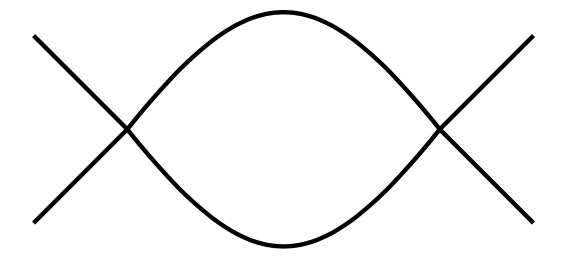
\includegraphics[align=c,width=0.15\linewidth]{pics/RG-2.jpg} 
	= \frac{g^{2}}{16} \int_{d\Lambda} \frac{d^{d} q}{(2 \pi)^{d}} \frac{1}{\left(r+q^{2}\right)^{2}} \left(\int d^{d} r\  \phi_{\mathrm{s}}^{4}\right).
\end{equation}
Similarly, the energy shell integral is
\begin{equation}
	\int_{d\Lambda} \frac{d^{d} q}{(2 \pi)^{d}} \frac{1}{\left(r+q^{2}\right)^{2}}
	= \int_{d\Lambda} \frac{d^{d} q}{(2 \pi)^{d}} \left(\frac{1}{q^4}-\frac{2r}{q^6} \right)
	= \Omega_d\left[\frac{1-s^{4-d}}{d-4}-\frac{2r(1-s^{6-d})}{d-6}\right].
\end{equation}
The RG-flow of $g$ is
\begin{equation}
\begin{aligned}
	dg &\rightarrow s^{(4-d)}\left[g - \frac{3g^2\Omega_d}{2(d-4)}(1-s^{4-d})+\frac{3rg^2\Omega_d}{d-6}(1-s^{6-d})\right]-g \\
	&\simeq [1+(4-d)dl] \left[g - \frac{3}{2} g^2\Omega_d dl + 3rg^2\Omega_d dl \right]-g \\
	&\simeq \left[(4-d)g-\frac{3}{2} g^2(1-2r)\Omega_d \right]dl.
\end{aligned}
\end{equation}
The beta function for lowest order $\varepsilon$-expansion is
\begin{equation}
	\frac{dg}{dl} = \varepsilon g - \frac{3g^2}{16\pi^2} + \frac{6 r g^2}{16\pi^2}.
\end{equation}

\begin{figure}[]
	\centering
	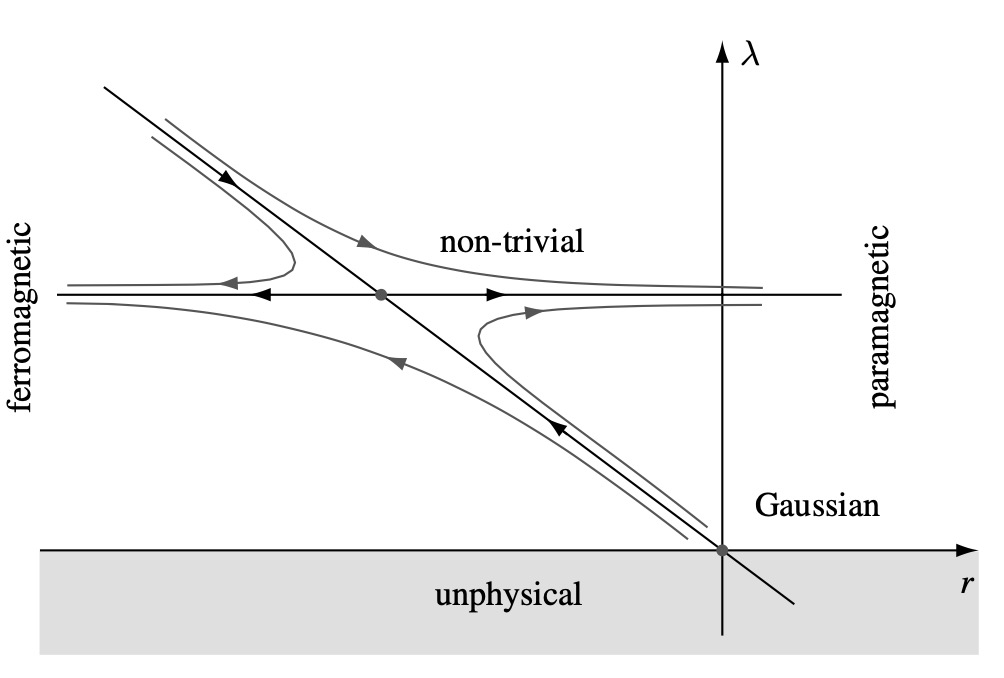
\includegraphics[hsmash=c,width=0.5\linewidth]{pics/RG-flow.jpg}
	\caption{Phase diagram of the $\phi^4$-model as obtained from the $\varepsilon$-expansion.}
	\label{fig:rg-flow}
\end{figure}

The Gaussian fixed point and the nontrivial Wilson-Fisher fixed point determined the phase diagram of the $\phi^4$ model.
As shown in Fig.~\ref{fig:rg-flow}, there are a disordered paramagnetic phase and an ordered ferromagnetic phase.
The ordered-disordered transition is the result of the spontaneous symmetry breaking.




\section{Spontaneous Symmetry Breaking}

In this section, we consider the effective field theory for the spontaneous symmetry breaking phase.
We first consider the real $\phi^4$ theory with $Z_2$ symmetry, then discuss the complex scalar field with continuous symmetry breaking.

\subsection{Spontaneous Breaking of $Z_2$ Symmetry}
The ferromagnetic phase correspond to the $\phi^4$ Lagrangian with minus mass term:
\begin{equation}
	\mathcal L =\frac{1}{2}\partial^\mu \phi \partial_\mu \phi +\frac{m^2}{2}\phi^2 - \frac{g}{4!}\phi^4.
\end{equation}
The energy is minimized by the nonzero field configuration
\begin{equation}
	\phi_0 = \pm \sqrt{\frac{6m^2}{g}}.
\end{equation}
To describe the low energy behavior, we just need to expand the field around on of the the minima: $\phi = \phi_0 +\tilde\phi$.
Then the effective theory is
\begin{equation}
	\mathcal{L}=\frac{1}{2} \partial_{\mu} \tilde{\phi}\partial^{\mu} \tilde{\phi} -m^{2} \tilde{\phi}^{2}-\sqrt{\frac{g}{6}} m \tilde{\phi}^{3}-\frac{g}{4 !} \tilde{\phi}^{4}+\frac{3 m^{4}}{2 g}.
\end{equation}
We see that the effective theory is an ordinary Klein-Gordon field with both $\phi^3$ and $\phi^4$ interaction present.
The original $Z_2$ symmetry $\phi \rightarrow -\phi$ is spontaneously broken. 


\subsection{Spontaneous Breaking of U(1) Symmetry}
Now we generalized the discussion the complex $\phi^4$ theory:
\begin{equation}
	\mathcal L = \partial^\mu \phi^* \partial_\mu \phi + m^2\phi^* \phi - \frac{g}{4}(\phi^*\phi)^2.
\end{equation}
The minimal energy field configuration is 
\begin{equation}
	|\phi_0|^2 = \frac{2m^2}{g}.
\end{equation}
The field can be parameterized as
\begin{equation}
	\phi(x)=\left[\sqrt{\frac{2 m^{2}}{g}}+\frac{\sigma(x)}{\sqrt{2}} \right] \exp\left[{i \frac{\pi(x)}{F_{\pi}}}\right],
\end{equation}
with $F_{\pi}$ a real number. 
Expanding the Lagrangian around the minimum we find
\begin{equation}
	\mathcal{L}= \frac{2m^2/g}{F_\pi^2} \left[1+\frac{\sqrt{g}}{2m} \sigma(x) \right]^{2} \left(\partial_{\mu} \pi\right)^{2} +\frac{1}{2}\left(\partial_{\mu} \sigma\right)^{2}
	-\left(m^{2} \sigma^{2}+\frac{\sqrt{g} m}{2} \sigma^{3}+\frac{g}{16} \sigma^{4}\right)+\frac{m^{4}}{g}.
\end{equation}
Choosing $F_\pi = 2m/\sqrt{g}$, the $\pi$ mode is canonically normalized.
This theory is called a \textit{linear sigma model}.
The massless $\pi$ field is the Goldstone boson.








\end{document}


